% TikZ codes by Le Huy Tien and Bui Quy
% For other TikZ/PGF, Asymptote code, see
% http://tikz.vn/vi/hinhve/mo-hinh-dia-poincare/
\documentclass[tikz,border=5mm]{standalone}
\usetikzlibrary{calc}
\newcommand{\geodesicarc}[4]
{
\def\R{#1} % radius of the big circle
\def\qone{#2} % start angle of the geodesic arc
\def\qtwo{#3} % end angle of the geodesic arc
\def\geodesiccolor{#4} % color of the geodesic arc

\pgfmathsetmacro{\f}{(\qtwo-\qone)/2}
\pgfmathsetmacro{\dq}{abs(\f)}
\pgfmathsetmacro{\r}{\R*tan(\dq)} % radius of the geodesic arc
\pgfmathsetmacro{\rp}{sqrt(\r*\r+\R*\R)} % distance of 2 centers 

\coordinate (I) at (\f+\qone:\rp);
\fill [color=\geodesiccolor] (I) circle (\r);
}% end of \geodesicarc command
\begin{document}
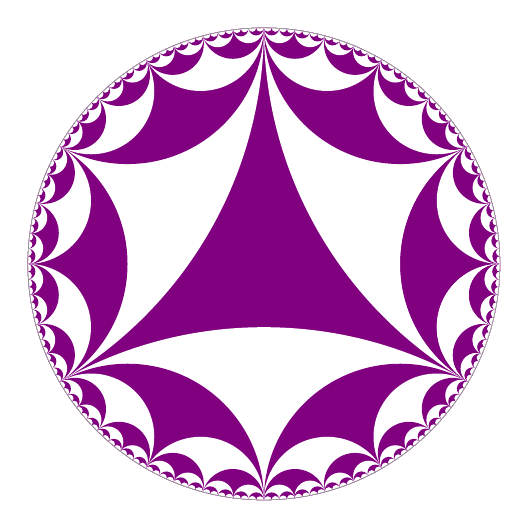
\begin{tikzpicture}
\def\RR{3} % radius of the Poincare's disk
\colorlet{Pdiskcolor}{violet} % color of the Poincare's disk

\clip (0:0) circle (\RR);
\fill[Pdiskcolor] (0,0) circle (\RR);

% Initiate geodesic triangle
\foreach \i in {-30,90,210}
\geodesicarc{\RR}{\i}{\i+120}{white};

% 1st iteration
\foreach \i in {-30,30,...,330}
\geodesicarc{\RR}{\i}{\i+60}{Pdiskcolor};

% 2nd iteration
\foreach \i in {-30,0,...,330}
\geodesicarc{\RR}{\i}{\i+30}{white};

% 3rd iteration
\foreach \i in {-30,-15,...,345}
\geodesicarc{\RR}{\i}{\i+15}{Pdiskcolor};

% 4th iteration
\foreach \i in {-30,-22.5,...,352.5}
\geodesicarc{\RR}{\i}{\i+7.5}{white};

% 5th iteration
\foreach \i in {-30,-26.25,...,356.25}
\geodesicarc{\RR}{\i}{\i+3.75}{Pdiskcolor};

% 6th iteration
\foreach \i in {-30,-28.125,...,358.125}
\geodesicarc{\RR}{\i}{\i+1.875}{white};

\draw[gray] (0,0) circle(\RR);
\end{tikzpicture} 
\end{document}